\section{Preliminaries}
The analysis combines two areas: black hole accretion physics and time-series causal discovery. The physical background explains why the Hard State and Soft State have different observational signatures. The statistical background explains how to model autocorrelation, hidden regime boundaries, and unknown state counts. This section introduces time-series concepts, causal inference, structural causal models, and the main tools used by the framework: OLS, the Chow test, binary segmentation, BIC, and DYNOTEARS.

\subsection{Multivariate Time-Series and Non-Stationarity}

\subsubsection*{i. Time Series Data}

Time-series data consist of observations collected at ordered time points. The order is part of the information in the data. A multivariate series can be written as $X = \{x_1, x_2, x_3, \dots, x_n\}$, where $n$ variables are measured over $T$ time steps \cite{assaad2022survey}. A variable at time $t$ may depend on variables from the same time step or on earlier observations. These past effects are called lagged effects. Because an infinite lag window is not practical, causal discovery uses a maximum lag, denoted by $I_{max}$.

\subsubsection*{ii. Stationary and Non-Stationary Data}

In stationary data, properties such as the mean and variance remain stable over time. In non-stationary data, these properties change, either gradually or at particular points.

\subsubsection*{iii. Temporal Regime}

A temporal regime is a consecutive time window in which the statistical properties or causal structure remain stable. If the properties are stable from $t=1$ to $t=m$ and change at $t=m+1$, the first interval forms one regime and the later stable interval up to $t=k$ forms another.

\subsubsection*{iv. Strict Stationary Assumption}

Many traditional models assume that the data-generating rules remain unchanged at every time step. This makes the time index independent of the data distribution and implies one causal structure for the whole series. The assumption is often unrealistic for dynamic systems. If the distribution or causal relationships change, a single stationary model can produce inaccurate or misleading discoveries.

\subsection{Black Holes and Accretion}

\subsubsection*{i. Black Holes}

Black holes are well-studied astrophysical objects, although many aspects of their behaviour remain uncertain.

A black hole is a region of spacetime from which light cannot escape after crossing the event horizon. Black holes are detected indirectly through their gravitational and electromagnetic effects on nearby matter. They can form when a massive star collapses. In general relativity, the event horizon marks the boundary beyond which information cannot return to an external observer.

For a non-rotating black hole, the radius of the event horizon is described by Equation~\eqref{eq:ch2-schwarzschild}:

\begin{equation}
    \label{eq:ch2-schwarzschild}
    R_s = \frac{2GM}{c^2}
\end{equation}

where $G$ is the gravitational constant, $M$ is the black-hole mass, and $c$ is the speed of light. At this radius, the escape velocity reaches the speed of light. The black hole itself does not emit electromagnetic radiation, but nearby matter can become very bright through \textit{accretion}.

\subsubsection*{ii. Accretion and Accretion Disks}

Accretion is the process by which matter is captured and moves toward a black hole. Because the matter has angular momentum, it usually forms a rotating flow instead of falling directly inward. Gravitational potential energy is converted into motion, heat, and radiation. Accretion is therefore one of the most efficient known mechanisms of energy release \cite{shakura1973, frank2002}.

As matter approaches a black hole, it forms a rotating accretion disk. Viscosity removes orbital energy and causes the gas to spiral inward. The resulting friction heats the disk to very high temperatures.

The disk is not equally hot at all radii. The outer region is cooler, while the inner region can emit strongly in X-rays. This emission provides information about the disk geometry and its behaviour.

\subsubsection*{iii. Black Hole X-ray Binaries}

Black holes are commonly grouped as \textit{stellar-mass}, \textit{intermediate-mass}, or \textit{supermassive}. Stellar-mass black holes in binary systems are common in the Milky Way. These systems are called Black Hole X-ray Binaries (BHXBs).

In a BHXB, the black hole orbits a companion star and pulls gas from it. The captured gas feeds the accretion disk. These systems allow rapid changes in accretion to be observed over weeks or months \cite{remillard2006, done2007}.
\subsubsection*{iv. Active Galactic Nuclei (AGN)}

\textit{Active Galactic Nuclei (AGN)} are powered by accretion onto supermassive black holes at the centres of galaxies. These black holes can be millions or billions of times more massive than the Sun.

The basic accretion physics is similar to that of stellar-mass black holes, but the larger mass produces much longer variability timescales. BHXBs can therefore serve as faster systems for studying accretion processes.

\subsubsection*{v. Accretion States}

Black holes do not accrete at a constant rate. They move between \textit{accretion states}, in which the flow geometry and energy-release mechanism change. The states are identified from their emitted spectra.

\subsubsection*{vi. Hard State}

In the \textit{Hard State}, the accretion rate is usually lower. The inner disk is often \textit{truncated} and replaced by a hot, diffuse gas cloud called a \textit{corona}.

A steady \textit{radio jet} is a key feature of this state. The observed emission is dominated by high-energy (\textit{Hard}) X-rays and often varies rapidly.

\subsubsection*{vii. Soft State}

At a higher accretion rate, the system can enter the \textit{Soft State}. The disk then extends inward to the closest stable orbit.

In the Soft State, the radio jet is \textit{quenched} or absent. The emission is dominated by thermal disk radiation and appears as a \textit{Soft} X-ray spectrum. Thus, the Soft State is disk-dominated, while the Hard State is jet-dominated.

\subsubsection*{viii. Power-Law Scaling Relations}

In contrast to the intricate physics of plasma dynamics and magnetic fields, the systems surrounding black holes exhibit a notable level of order. They adhere to Power-Law Scaling Relations. One physical feature (like brightness) is proportional to another raised to a specific exponent, $y = A x^k$.

In science, power laws are often a sign of scale \textit{invariance}. This suggests that the same physical law applies whether the black hole is small or supermassive. For the purpose of this research, these relations are very important because power laws become linear when converted to a logarithmic scale ($\log y = k \log x + \log A$). This makes them ideal for the causal discovery methods explored here.

\subsubsection*{ix. Fundamental Plane of Black Hole Activity}

The \textit{Fundamental Plane of Black Hole Activity} is a specific scaling relation that serves as a "universal rulebook" for black hole physics \cite{merloni2003}. It connects three core properties: Radio luminosity ($L_R$), X-ray luminosity ($L_X$), and the mass of the black hole ($M_{BH}$). Empirical observations indicate that the physical processes involved in accretion and jet production are similar over several orders of magnitude in mass:

Equation~\eqref{eq:ch2-fp-power} gives the power-law form:
\begin{equation}
    \label{eq:ch2-fp-power}
    L_R \propto L_X^{\xi_X} M_{BH}^{\xi_M}
\end{equation}

This relation is expressed logarithmically in Equation~\eqref{eq:ch2-fp-log}:

\begin{equation}
    \label{eq:ch2-fp-log}
    \log L_R = a \log L_X + b \log M_{BH} + c
\end{equation}

\subsection{Fundamentals of Causal Inference}

\textit{To understand the mechanisms governing each temporal regime, we rely on the formal framework of causal inference. This section introduces the necessary graphical and structural definitions, adopting the framework detailed by Neal (2020).}

\subsubsection*{i. Directed Acyclic Graphs (DAGs)}

A \textit{graph} is a mathematical structure consisting of a set of \textit{nodes} (or vertices) and a set of \textit{edges}, where each edge represents a relationship between two nodes. In the context of causal inference, nodes represent the variables or features of the dataset \cite{neal2020}.

In a \textit{directed graph}, edges contain arrows indicating the direction of the relationship. The node from which an edge originates is called the \textit{parent} node, and the node the edge points to is called the \textit{child} node. 

A \textit{path} is a sequence of nodes connected by edges, regardless of the direction of the arrows. A \textit{directed path}, however, is a sequence of nodes connected by directed edges that all point in the same forward direction. 

For a given node $X$, its \textit{descendants}, denoted as $de(X)$, consist of all nodes $Y$ for which there exists a directed path from $X$ to $Y$ (this includes children, children of children, and so forth). 
Conversely, the \textit{ancestors} of $Y$, denoted as $an(Y)$, consist of all nodes $X$ for which there exists a directed path from $X$ to $Y$ (including parents, parents of parents, etc.).

A \textbf{Directed Acyclic Graph (DAG)} is a directed graph that contains no \textit{cycles}; namely, there does not exist any directed path that starts and ends at the same node. Consequently, no node can be an ancestor or descendant of itself \cite{neal2020}.

\subsubsection*{ii. Causal Graphs}

A variable $X$ is considered a \textit{cause} of a variable $Y$ if an intervention or deliberate change in $X$ results in a change in the distribution of $Y$; this underlying mechanism is referred to as \textit{causation} \cite{neal2020}.

Within the framework of a directed graph, the \textit{Causal Edges Assumption} states that every parent node is a direct cause of all its child nodes. 

Consequently, a \textbf{Causal Graph} is formally defined as a Directed Acyclic Graph (DAG) that strictly satisfies the Causal Edges Assumption. In such a graph, every directed path from one node to another implies a flow of causation.

\subsubsection*{iii. Statistical Independence and Dependence}

Two random variables $X$ and $Y$ are \textbf{statistically independent} (or marginally independent), denoted as $X \perp\!\!\!\perp Y$, if their joint probability satisfies Equation~\eqref{eq:ch2-independence}:
\begin{equation}
    \label{eq:ch2-independence}
    P(X=x, Y=y) = P(X=x)P(Y=y)
\end{equation}
If this equality does not hold for at least one pair of $(x, y)$, the variables are \textbf{statistically dependent}, denoted as $X \not\perp\!\!\!\perp Y$, implying that observing the value of $X$ provides information that changes the probability of $Y$.

In real-life systems, variables are rarely entirely independent. Instead, we rely on \textbf{conditional independence}. Two random variables $X$ and $Y$ are conditionally independent given a third variable (or set of variables) $Z$, denoted as $X \perp\!\!\!\perp Y \mid Z$, if Equation~\eqref{eq:ch2-cond-independence} holds:
\begin{equation}
    \label{eq:ch2-cond-independence}
    P(X=x, Y=y \mid Z=z) = P(X=x \mid Z=z)P(Y=y \mid Z=z)
\end{equation}
In causal terms, conditional independence implies that once $Z$ is known, observing $X$ provides no additional information about $Y$ \cite{wasserman2004}.

\subsubsection*{iv. d-Separation and the Flow of Association}

In a causal graph, it is necessary to understand the conditional independence or dependence between two nodes. This criterion is known as \textbf{d-separation} (directional separation) \cite{neal2020}. 

Two nodes $X$ and $Y$ are d-separated by a set of conditioning nodes $Z$ if all paths between $X$ and $Y$ are mathematically blocked by $Z$. If $X$ and $Y$ are d-separated in the graph $\mathcal{G}$, it implies they are conditionally independent in the probability distribution: $X \perp\!\!\!\perp Y \mid Z$. Note that $Z$ is a set of nodes which can be empty.

To determine whether a specific path is open or blocked, we evaluate the path using three structural building blocks \cite{neal2020}:

\begin{quote}
\textbf{1. Chains (Mediation)}\\
A chain represents a sequence where causation flows through an intermediate variable ($X \rightarrow Z \rightarrow Y$). Here, $X$ is a cause of $Z$, and $Z$ is a cause of $Y$.
This path is by default open and $X$ and $Y$ are statistically dependent. However, conditioning on the mediator $Z$ blocks the flow of association. 
\textit{Example:} In urban infrastructure, heavy rain ($X$) causes waterlogging ($Z$), which subsequently causes severe traffic gridlock ($Y$). Conditioning on the waterlogging ($Z$) mathematically blocks the association between heavy rain and traffic gridlock.

\begin{center}
\begin{tikzpicture}[->, >=stealth, thick, node distance=2cm]
    \node[circle, draw, minimum size=0.8cm] (X) {$X$};
    \node[circle, draw, minimum size=0.8cm] (Z) [right=of X] {$Z$};
    \node[circle, draw, minimum size=0.8cm] (Y) [right=of Z] {$Y$};
    \draw (X) -- (Z);
    \draw (Z) -- (Y);
\end{tikzpicture}
\end{center}
\end{quote}

\begin{quote}
\textbf{2. Forks (Confounding)}\\
A fork happens when a single variable is the common cause of two separate variables ($X \leftarrow Z \rightarrow Y$). Here, $Z$ is a cause of both $X$ and $Y$.
This path is open by default, introducing confounding bias. Conditioning on the common cause $Z$ blocks this spurious flow of association.
\textit{Example:} A summer heatwave ($Z$) simultaneously causes load-shedding ($X$) and an increase in app-based ride demand ($Y$). Conditioning on the temperature ($Z$) d-separates the electricity usage from the ride-hailing demand, removing the fake correlation between load-shedding ($X$) and app-based ride demand ($Y$).

\begin{center}
\begin{tikzpicture}[->, >=stealth, thick, node distance=2cm]
    \node[circle, draw, minimum size=0.8cm] (Z) {$Z$};
    \node[circle, draw, minimum size=0.8cm] (X) [below left=1cm and 1cm of Z] {$X$};
    \node[circle, draw, minimum size=0.8cm] (Y) [below right=1cm and 1cm of Z] {$Y$};
    \draw (Z) -- (X);
    \draw (Z) -- (Y);
\end{tikzpicture}
\end{center}
\end{quote}

\begin{quote}
\textbf{3. Colliders (Selection Bias)}\\
A collider exists when two independent variables have a common effect ($X \rightarrow Z \leftarrow Y$). Here, both $X$ and $Y$ are causes of $Z$. If $X$ and $Y$ are not directly connected by an edge, this specific V-structure is formally known as an \textit{immorality}. 
Unlike chains and forks, a collider naturally blocks the flow of association. However, conditioning on the collider $Z$ (or any of its descendants) opens a spurious path between $X$ and $Y$. 
\textit{Example:} In an academic environment, consider the factors for getting a good grade in a certain course ($Z$). A student's prior foundational knowledge ($X$) and their dedicated study hours ($Y$) independently increase the probability of securing an 'A'. Prior knowledge and study hours might be independent; however, if a researcher restricts their analysis to students who actually received an 'A' (conditioning on the collider $Z$), they will induce a spurious negative correlation. Within this conditioned group, a student without prior foundational knowledge must have compensated with a high number of study hours to achieve the grade. This creates a mathematically false implication that having stronger foundational knowledge causes a student to study less. 

\begin{center}
\begin{tikzpicture}[->, >=stealth, thick, node distance=2cm]
    \node[circle, draw, minimum size=0.8cm] (Z) {$Z$};
    \node[circle, draw, minimum size=0.8cm] (X) [above left=1cm and 1cm of Z] {$X$};
    \node[circle, draw, minimum size=0.8cm] (Y) [above right=1cm and 1cm of Z] {$Y$};
    \draw (X) -- (Z);
    \draw (Y) -- (Z);
\end{tikzpicture}
\end{center}
\end{quote}

Formally, a path between nodes $A$ and $B$ is blocked (no flow of association) by a conditioning set $M$ if at least one of the following conditions is met \cite{neal2020}:
\begin{enumerate}
    \item The path contains a chain ($X \rightarrow Y \rightarrow Z$) or a fork ($X \leftarrow Y \rightarrow Z$) such that the middle node $Y$ is in the conditioning set $M$.
    \item The path contains a collider ($X \rightarrow Y \leftarrow Z$) such that the middle node $Y$ is \textit{not} in $M$, and no descendant of $Y$ is in $M$.
\end{enumerate}

\subsubsection*{v. Structural Causal Models (SCMs)}

A \textbf{Structural Causal Model (SCM)} is a mathematical framework used to model cause-and-effect relations in an environment \cite{neal2020}. While a DAG is the visual description of causality, an SCM provides the mathematical rules for those relations. 

In an SCM, every single node is calculated through the function in Equation~\eqref{eq:ch2-scm}:
\begin{equation}
    \label{eq:ch2-scm}
    X_i := f_i(\text{PA}(X_i), \epsilon_i)
\end{equation}
where: 
\begin{itemize}
    \item $X_i$ (The effect): The variable being calculated.
    \item $\text{PA}(X_i)$ (The causes): The set of parents of $X_i$ which are causing the effect.
    \item $f_i$ (The function): The deterministic mathematical relation that computes the effect from the causes.
    \item $\epsilon_i$ (The noise term): The variation in the effect that the causes \textit{cannot} explain.
    \item $:=$ (The assignment): The mathematical assignment operation means $X_i$ is defined by the right-hand side. Note that this operation is not symmetric. 
\end{itemize}

To illustrate how a DAG translates into structural mathematical equations, consider a system with the causal structure: $A \rightarrow C$, $B \rightarrow C$, $B \rightarrow D$, $D \rightarrow E$, and $E \rightarrow F$.

\begin{center}
\begin{tikzpicture}[->, >=stealth, thick, node distance=1.5cm]
    \node[circle, draw] (A) {$A$};
    \node[circle, draw] (B) [below=of A] {$B$};
    \node[circle, draw] (C) [right=of A] {$C$};
    \node[circle, draw] (D) [right=of B] {$D$};
    \node[circle, draw] (E) [right=of D] {$E$};
    \node[circle, draw] (F) [right=of E] {$F$};
    \draw (A) -- (C);
    \draw (B) -- (C);
    \draw (B) -- (D);
    \draw (D) -- (E);
    \draw (E) -- (F);
\end{tikzpicture}
\end{center} 

The corresponding SCM defines each node as a deterministic function of its direct parents and its unobserved noise ($\epsilon$): 
\begin{align*}
A &:= f_A(\epsilon_A) \\
B &:= f_B(\epsilon_B) \\
C &:= f_C(A, B, \epsilon_C) \\
D &:= f_D(B, \epsilon_D) \\
E &:= f_E(D, \epsilon_E) \\
F &:= f_F(E, \epsilon_F)
\end{align*}

In this structure, nodes $A$ and $B$ have no direct parents (they act as root nodes), meaning their assignments rely entirely on their respective noise terms. Node $C$, acting as a collider between $A$ and $B$, takes both parent variables as arguments in its structural function.

\subsubsection*{vi. The Discovery Postulates: Markov and Faithfulness}

Every mathematical field stands on axioms and postulates. Similarly, to successfully discover a causal graph $\mathcal{G}$ from the probability distribution $P$ of observational data, it is necessary to establish a mathematical bridge between the SCM and statistical independence. This bridge relies on two foundational postulates: the \textbf{Causal Markov Assumption} and the \textbf{Faithfulness Assumption} \cite{neal2020}.

\begin{quote}
\textbf{1. The Local Causal Markov Assumption} (Equation~\eqref{eq:ch2-markov})\\
The Causal Markov Assumption dictates that a node is conditionally independent of all its non-descendants, given its direct parents. Formally, for any node $X$ in a DAG $\mathcal{G}$, where $\text{PA}(X)$ represents its parents and $\text{ND}(X)$ represents its non-descendants:
\begin{equation}
    \label{eq:ch2-markov}
    X \perp\!\!\!\perp \text{ND}(X) \mid \text{PA}(X)
\end{equation}
This assumption guarantees that the causal graph naturally imposes the correct conditional independencies on the joint probability distribution. If two variables are d-separated in the graph $\mathcal{G}$, they \textit{must} be statistically independent in the data $P$.
\end{quote}

\begin{quote}
\textbf{2. The Faithfulness Assumption}\\
The Faithfulness Assumption is the logical converse of the Markov Assumption. A probability distribution $P$ is considered faithful to a DAG $\mathcal{G}$ if \textit{every} conditional independence observed in the data is strictly the result of a structural d-separation in the graph.
Formally, if $X \perp\!\!\!\perp Y \mid Z$ is found in the data distribution $P$, then $X$ and $Y$ must be d-separated by $Z$ in $\mathcal{G}$. This axiom ensures that two causal paths do not perfectly and coincidentally cancel each other out to create a fake statistical independence.
\end{quote}

Together, these postulates guarantee that the structural d-separations in the causal graph perfectly map to the statistical conditional independencies in the observable time-series data, making the unsupervised discovery of the DAG mathematically possible.


\subsection{Unsupervised Learning and Clustering}

\textit{Because the structural boundaries of real-world temporal regimes are rarely known in advance, discovering these shifts requires analyzing the data without predefined labels. This section discusses the application of clustering and temporal segmentation to identify these hidden causal boundaries.}

\subsubsection*{i. The Need for Unsupervised Learning}

We have theoretically established the basic theoretical framework for modeling causal structure. In this section, we address a major methodological challenge of causal modeling, which is detecting the temporal regimes without knowing the structural boundaries of the data. We frame this as an unsupervised learning problem. In traditional supervised learning algorithms, models are trained with data with input features $x$ where the actual outputs $y$ are known beforehand. But in most real-life dynamic systems, it is not feasible to gather the predefined target outputs. So, the exact boundaries of the temporal regimes stay hidden. Supervised learning cannot work in this case. To solve this, we rely on unsupervised learning, which seeks to recover latent structure without reference to known or labeled outcomes \cite{hastie2009}. Since our multivariate time-series data does not contain the predefined labels, it is mandatory to use unsupervised learning to discover the underlying Structural Causal Model (SCM) shifts.

\subsubsection*{ii. Clustering vs. Temporal Segmentation}

One of the primary techniques for unsupervised learning is the method of clustering. In this method, the data are grouped in a way such that the intra-group similarity is maximized and the inter-group similarity is minimized. One such well-known clustering technique is k-means clustering. In this method, data points are assigned to clusters based entirely on their feature proximity, ignoring the sequence of the data. So, applying standard clustering on time-series data where the sequence matters destroys the temporal precedence required for causal discovery. To solve this problem, we can use temporal segmentation. Temporal segmentation safeguards continuity by grouping contiguous time blocks into discrete clusters. Here, each cluster represents a temporal regime, and the boundary between two regimes is now clearly defined, which our causal model may work with \cite{assaad2022survey}. 

To illustrate this within a real-world context, consider the highly dynamic environmental and traffic conditions of Dhaka City. A multivariate time-series dataset tracking hourly parameters, such as traffic density, weather metrics (humidity, wind speed), and air quality markers like PM2.5, exhibits distinct, unlabeled temporal regimes. During the Winter Regime (November-February), cold weather and stagnant air mean traffic density has a strong, direct causal link to sudden PM2.5 spikes. However, during the Monsoon Regime (June-August), heavy rainfall washes away pollutants, breaking or heavily weakening that direct causal link, while the rain itself becomes the primary cause of traffic gridlock. Standard clustering like k-means would completely ignore this and may group data based only on features like traffic speed, which may cluster winter data and summer data together. Temporal segmentation, however, treats winter and monsoon as continuous, separate blocks of time with their own distinct causal behaviors.

\subsubsection*{iii. Requirements for Temporal Segmentation}

Although there exist many algorithms which may be used to perform temporal segmentation, some rules or requirements have to be enforced for our specific problem.

\begin{itemize}
    \item \textbf{Contiguity enforcement:} The algorithm must ensure that each cluster is an unbroken sequence of time. 
    \item \textbf{Dynamic graph optimization:} The cluster fit shouldn't just be the distance between two data points, but also how a Directed Acyclic Graph (DAG) explains the entire block of data. 
    \item \textbf{Complexity penalization:} The algorithm might assign each time-step its own unique regime which we have to prevent. We can prevent it by ensuring that some penalty term is added to the objective function which balances the accuracy of the causal graph against the number of structural breaks. 
\end{itemize}

By satisfying the requirements, the unsupervised algorithm can successfully divide the non-stationary time-series data into unique stationary regimes, which will allow the discovery of a DAG within each time block.


\subsection{Dynamic Causal Models and Time-Series Graphs}

In a standard Structural Causal Model (SCM), cause-and-effect relationships are captured only at a single, isolated instant. The underlying mathematics cannot account for historical dependencies, and a traditional DAG is limited to representing static relations. To evaluate dynamical systems, causal influences from the past must be explicitly taken into account. Therefore, to properly study structural breaks across temporal regimes, we must shift from the standard causal framework introduced in the previous section to Dynamic Causal Models.

\subsubsection*{i. Unrolling the Graph over Time (Dynamic Bayesian Networks)}

A Dynamic Bayesian Network (DBN) is a directed graphical representation of a stochastic process \cite{murphy2012}. It is important to note that the network structure itself is not dynamic; rather, it is a fixed topology that models variables across discrete slices of time. By unrolling these static time slices, the network formally represents a dynamical system capable of accounting for historical dependencies. 

To rigorously define a DBN, three structural requirements must be specified \cite{murphy2012}:
\begin{enumerate}
    \item \textbf{The Initial State:} The structural topology of the first time-slice ($t = 0$).
    \item \textbf{The Transition Model:} The directed connections between historical time-slices ($t - \tau$) and the current time-slice ($t$).
    \item \textbf{The Probability Distributions:} The specific Conditional Probability Distributions (CPDs) that mathematically govern the relations along these directed connections.
\end{enumerate}

\subsubsection*{ii. Defining Time-Series Causal Graphs}

To apply causal discovery algorithms to time-series data, we must mathematically formalize how the unrolled Dynamic Bayesian Network is represented as a graph. Depending on the level of temporal detail required, time-series causality can be represented using three distinct graphical definitions \cite{assaad2022survey}. These representations are illustrated in Figure~\ref{fig:timeseries-graphs}:

\begin{quote}
\textbf{1. The Full Time Causal Graph}\\
The Full Time Causal Graph captures all causal relations throughout all possible time. This is an infinite Directed Acyclic Graph (DAG) where every variable at every time step is denoted by an independent node.  
Formally, the set of nodes is defined as $\{X_t^i \mid \forall i, \forall t \}$. An edge drawn from $X_{t-\tau}^j \rightarrow X_t^i$ indicates a direct causal relationship with an exact time delay of $\tau$. If $\tau = 0$, the edge represents a contemporaneous effect; if $\tau > 0$, the edge represents a lagged effect. 
Although this graph contains all the theoretical information, the sheer number of nodes and edges makes it computationally intractable for causal discovery algorithms.   
\end{quote}

\begin{quote}
\textbf{2. The Window Causal Graph}\\
Because the Full Time Causal Graph is computationally intractable, we must compress the temporal information into a manageable window. As a result, this graph restricts the analysis to a specific, finite maximum time lag, denoted as $\tau_{max}$. 
In this representation, an edge $X_{t-\tau}^j \rightarrow X_t^i$ is only valid and included in the graph if the delay is within the sliding window ($\tau \leq \tau_{max}$). This operates under the assumption that an effect past $\tau_{max}$ is negligible and is instead mediated by more recent causal relations. The Window Causal Graph is the primary target structure for time-series causal discovery algorithms and is the most prominent representation utilized in this thesis. 
\end{quote}

\begin{quote}
\textbf{3. The Summary Causal Graph}\\
Unlike the Full Time Causal Graph or the Window Causal Graph, the Summary Causal Graph does not incorporate timestamps; it serves as a full summary of the entire temporal history, containing information across all time steps. In this graph, nodes revert to their static definitions ($X^i$ and $X^j$, dropping the time index $t$). 
An edge $X^j \rightarrow X^i$ is drawn if there exists \textit{any} time delay $\tau \geq 0$ where $X_{t-\tau}^j$ causes $X_t^i$ in the underlying full graph. Because this aggregation ignores the strict forward-flowing direction of time, a Summary Causal Graph can contain cycles ($X^j \rightarrow X^i$ and $X^i \rightarrow X^j$ can simultaneously exist if they occur at different lags). Therefore, unlike a standard static causal graph, a Summary Causal Graph is not necessarily a DAG.
\end{quote}

\begin{figure}[h!]
\centering
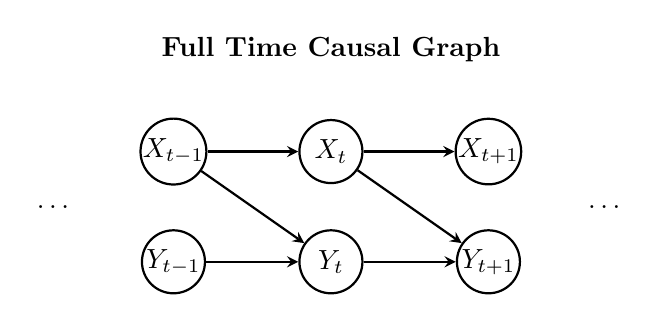
\begin{tikzpicture}[->, >=stealth, thick, node distance=1.5cm]
    % Full Time Causal Graph
    \node (FT_title) at (3.5, 2) {\textbf{Full Time Causal Graph}};
    \node (t0) at (0,0) {\dots};
    \node[circle, draw, minimum size=0.8cm, inner sep=0pt] (X1) at (1.5, 0.7) {$X_{t-1}$};
    \node[circle, draw, minimum size=0.8cm, inner sep=0pt] (Y1) at (1.5, -0.7) {$Y_{t-1}$};
    \node[circle, draw, minimum size=0.8cm, inner sep=0pt] (X2) at (3.5, 0.7) {$X_{t}$};
    \node[circle, draw, minimum size=0.8cm, inner sep=0pt] (Y2) at (3.5, -0.7) {$Y_{t}$};
    \node[circle, draw, minimum size=0.8cm, inner sep=0pt] (X3) at (5.5, 0.7) {$X_{t+1}$};
    \node[circle, draw, minimum size=0.8cm, inner sep=0pt] (Y3) at (5.5, -0.7) {$Y_{t+1}$};
    \node (t4) at (7,0) {\dots};

    \draw (X1) -- (X2); \draw (X2) -- (X3);
    \draw (Y1) -- (Y2); \draw (Y2) -- (Y3);
    \draw (X1) -- (Y2); \draw (X2) -- (Y3);
\end{tikzpicture}

\vspace{1cm}

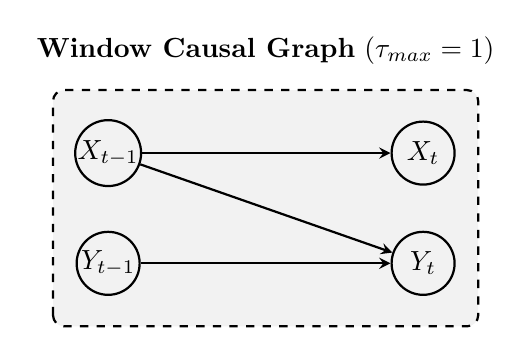
\begin{tikzpicture}[->, >=stealth, thick, node distance=1.5cm]
    % Window Causal Graph
    \node (W_title) at (2, 2) {\textbf{Window Causal Graph} ($\tau_{max} = 1$)};
    \draw[dashed, fill=gray!10, rounded corners] (-0.7, -1.5) rectangle (4.7, 1.5);
    \node[circle, draw, minimum size=0.8cm, inner sep=0pt] (X1) at (0, 0.7) {$X_{t-1}$};
    \node[circle, draw, minimum size=0.8cm, inner sep=0pt] (Y1) at (0, -0.7) {$Y_{t-1}$};
    \node[circle, draw, minimum size=0.8cm, inner sep=0pt] (X2) at (4, 0.7) {$X_{t}$};
    \node[circle, draw, minimum size=0.8cm, inner sep=0pt] (Y2) at (4, -0.7) {$Y_{t}$};
    \draw (X1) -- (X2);
    \draw (Y1) -- (Y2);
    \draw (X1) -- (Y2);
\end{tikzpicture}

\vspace{1cm}

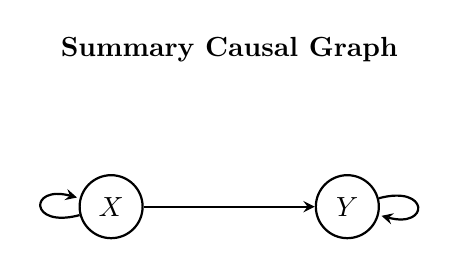
\begin{tikzpicture}[->, >=stealth, thick, node distance=2cm]
    % Summary Causal Graph
    \node (S_title) at (1.5, 2) {\textbf{Summary Causal Graph}};
    \node[circle, draw, minimum size=0.8cm] (X) at (0, 0) {$X$};
    \node[circle, draw, minimum size=0.8cm] (Y) at (3, 0) {$Y$};
    \draw (X) edge[loop left] (X);
    \draw (Y) edge[loop right] (Y);
    \draw (X) -- (Y);
\end{tikzpicture}
\caption{Representations of Time-Series Causal Graphs}
\label{fig:timeseries-graphs}
\end{figure}

By understanding these three representations, we can define unsupervised clustering algorithms to discover distinct temporal regimes in a time-series by analyzing localized Window or Summary Causal Graphs.

\subsubsection*{iii. The Time-Series Structural Causal Model}

A standard Structural Causal Model (SCM) assumes all variables operate within the same isolated instant. However, in a Time-Series Structural Causal Model, we must extend this framework to account for the flow of time $t$.

In a time-series SCM, a variable is not merely caused by other variables, but by specific historical time instants (from $t-1$ down to $t - \tau_{max}$) of those variables \cite{assaad2022survey}. Equation~\eqref{eq:ch2-timeseries-scm} formally defines a time-series SCM:

\begin{equation}
    \label{eq:ch2-timeseries-scm}
    X_t^i := f_i( \{ X_{t-\tau}^j \mid X_{t-\tau}^j \in \text{PA}(X_t^i) \}, \epsilon_t^i )
\end{equation}

where:
\begin{itemize}
    \item $X_t^i$ (The present effect): The target variable being calculated at the current time step $t$.
    \item $\text{PA}(X_t^i)$ (The temporal parents): The set of all direct causes of $X_t^i$. Because time is now a factor, this set can contain two distinct types of causes:
    \begin{itemize}
        \item \textbf{Contemporaneous Effects:} Causes that occur within the exact same time step ($\tau = 0$), denoted as $X_t^j \rightarrow X_t^i$.
        \item \textbf{Time-Lagged Effects:} Causes that occurred in the strict past ($\tau > 0$), denoted as $X_{t-\tau}^j \rightarrow X_t^i$. Note that a variable can be a lagged cause of itself ($X_{t-\tau}^i \rightarrow X_t^i$), representing auto-correlation.
    \end{itemize}
    \item $f_i$: The deterministic function mapping the historical and instantaneous parents to the current effect.
    \item $\epsilon_t^i$: The independent noise term at time $t$.
\end{itemize}

To illustrate how a static DAG is unrolled into this time-series SCM format (using a maximum time lag of $\tau_{max} = 2$), consider a dynamic system with three variables ($A$, $B$, and $C$). Let the causal structure dictate the following temporal rules: $A$ influences its own next state, $A$ influences $B$ with a delay of two time steps, $B$ influences its own next state, $A$ influences $C$ with a delay of one time step, and $B$ influences $C$ instantaneously.

\begin{center}
\begin{tikzpicture}[->, >=stealth, thick, node distance=2cm]
    % time t-2
    \node[circle, draw, inner sep=1pt, minimum size=0.8cm] (A2) at (0, 2) {$A_{t-2}$};
    \node[circle, draw, inner sep=1pt, minimum size=0.8cm] (B2) at (0, 0) {$B_{t-2}$};
    \node[circle, draw, inner sep=1pt, minimum size=0.8cm] (C2) at (0, -2) {$C_{t-2}$};

    % time t-1
    \node[circle, draw, inner sep=1pt, minimum size=0.8cm] (A1) at (3, 2) {$A_{t-1}$};
    \node[circle, draw, inner sep=1pt, minimum size=0.8cm] (B1) at (3, 0) {$B_{t-1}$};
    \node[circle, draw, inner sep=1pt, minimum size=0.8cm] (C1) at (3, -2) {$C_{t-1}$};

    % time t
    \node[circle, draw, inner sep=1pt, minimum size=0.8cm] (A0) at (6, 2) {$A_{t}$};
    \node[circle, draw, inner sep=1pt, minimum size=0.8cm] (B0) at (6, 0) {$B_{t}$};
    \node[circle, draw, inner sep=1pt, minimum size=0.8cm] (C0) at (6, -2) {$C_{t}$};

    % Column labels
    \node[above=0.5cm of A2, font=\bfseries] {Time $t-2$};
    \node[above=0.5cm of A1, font=\bfseries] {Time $t-1$};
    \node[above=0.5cm of A0, font=\bfseries] {Time $t$};

    % Rules applied sequentially to represent DBN
    % A auto-correlation
    \draw (A2) -- (A1);
    \draw (A1) -- (A0);
    
    % B auto-correlation
    \draw (B2) -- (B1);
    \draw (B1) -- (B0);
    
    % A influences B with lag 2
    \draw (A2) -- (B0);
    
    % A influences C with lag 1
    \draw (A2) -- (C1);
    \draw (A1) -- (C0);
    
    % B influences C instantaneously
    \draw (B2) -- (C2);
    \draw (B1) -- (C1);
    \draw (B0) -- (C0);

\end{tikzpicture}
\end{center} 

The corresponding time-series equations dictate the state of each node at the current time step $t$:

\begin{align*}
A_t &:= f_A(A_{t-1}, \epsilon_{A,t}) \\
B_t &:= f_B(B_{t-1}, A_{t-2}, \epsilon_{B,t}) \\
C_t &:= f_C(B_t, A_{t-1}, \epsilon_{C,t})
\end{align*}

In this dynamic system, the equation for $A_t$ demonstrates a lagged auto-correlation ($\tau = 1$), the equation for $B_t$ demonstrates a cross-lagged effect reaching back to the maximum lag limit ($\tau = 2$), and the equation for $C_t$ demonstrates a combination of a historical effect from $A$ ($\tau = 1$) and a contemporaneous effect from $B$ ($\tau = 0$).

\subsubsection*{iv. Consistency Throughout Time and Structural Breaks}

The mathematical formalizations of Time-Series SCMs and Window Causal Graphs rely on a fundamental assumption: the underlying causal mechanisms do not change spontaneously or erratically. It is highly unlikely that a causal direction will abruptly flip within a stable window; if such instability occurred frequently, the system would fragment into countless micro-regimes, causing the predictive model to collapse. In most macroscopic real-world scenarios, a causal link from $A$ to $B$ might weaken or disappear over time, but an immediate reversal where $B$ suddenly causes $A$ is highly improbable. This principle of stability is formally known as \textbf{Consistency Throughout Time}.

According to Assaad et al. \cite{assaad2022survey}, a time-series causal graph is consistent throughout time if the presence and direction of every causal edge remain invariant across all time steps. For instance, if $X$ causes $Y$ with a lag of $\tau = 1$ at time $t$, it must also cause $Y$ with the exact same lag at time $t+100$. 

In the context of this thesis, Consistency Throughout Time serves as the core defining characteristic of a \textbf{Temporal Regime}. As long as the consistency of the causal graph remains unbroken, that contiguous block of time constitutes a single, independent regime. 

However, in real-world dynamical systems, environments evolve and underlying rules change. When this consistency assumption is violated over time—for example, when an existing causal edge disappears or a new one emerges—we denote that exact moment as a \textbf{Structural Break}. Consequently, the time steps following this break transition into an entirely different regime. In observational data, this often manifests as certain variables becoming causally isolated while new cause-and-effect relationships are born.

To illustrate this dynamically, we extend the Dhaka City environmental model introduced in Section 2.1.4. Consider a multivariate time-series dataset tracking hourly parameters: Traffic Density ($X$), PM2.5 levels ($Y$), and Rainfall ($Z$). 

\begin{itemize}
    \item \textbf{Regime 1: The Winter Consistency (Nov--Feb):} Cold weather and stagnant air mean traffic density has a strong, direct causal link to sudden PM2.5 spikes. During this contiguous block of time, the Window Causal Graph maintains a perfectly consistent, lagged edge: $X_{t-\tau} \rightarrow Y_t$.
    \item \textbf{The Structural Break:} As the climate shifts, the environmental physics governing the city fundamentally change. The consistency assumption is violated.
    \item \textbf{Regime 2: The Monsoon Consistency (Jun--Aug):} Heavy rainfall washes away pollutants, effectively breaking the direct causal link from traffic to air quality. Simultaneously, the rain itself becomes the primary cause of traffic gridlock. The old causal edge ($X_{t-\tau} \rightarrow Y_t$) disappears from the Window Causal Graph, replaced by a newly consistent edge representing the rain's effect on traffic ($Z_{t-\tau} \rightarrow X_t$).
\end{itemize}

Because the exact temporal boundary (the structural break) between these distinct causal regimes is hidden within the unlabeled observational data, we cannot rely on supervised learning to locate it. This dictates the core methodological approach of this thesis: we must treat the discovery of these structural breaks as an \textbf{unsupervised learning} problem, utilizing clustering algorithms to segment the time-series based solely on the shifting structures of the underlying Window Causal Graphs.


\subsection{Algorithmic Framework for Regime Detection and Causal Discovery}

Identifying independent temporal regimes, and more precisely, locating their underlying structural breaks require a multi-step pipeline. Therefore, our methodology relies on the integration of multiple algorithms, analytical tools, and optimization techniques. Within this pipeline, the time-series data is first segmented into distinct temporal regimes, and subsequently, the specific causal structure of each isolated regime is extracted. To achieve this, our framework relies on three core stages:

\subsubsection*{i. Parameter Estimation and Model Scoring}
\begin{itemize}
    \item \textbf{Ordinary Least Squares (OLS):} OLS serves as the baseline optimization technique in this framework. It mathematically estimates the strength of the relationship (the edge weight) between a historical cause and a present effect. Because these cause-and-effect relationships are temporal, the true edge weights remain constant within a stable regime but shift when a structural break occurs. By minimizing the residual sum of squares, OLS evaluates the baseline error for any given window of time.  
    \item \textbf{Bayesian Information Criterion (BIC):} BIC acts as the penalized scoring metric for this framework. During clustering, if every tiny chunk of time were segmented independently, the OLS error would drop to near zero, but the model would severely overfit, rendering the results meaningless. BIC introduces a mathematical penalty for each new regime discovered. Consequently, it balances the need to minimize OLS error against model complexity, ensuring the algorithm does not fracture the timeline into an excessive and insignificant number of segments.  
\end{itemize}

This fundamental trade-off between minimizing OLS error and minimizing the BIC penalty ensures the mathematical foundation necessary to deploy search algorithms to locate the exact structural breaks.

\subsubsection*{ii. Structural Break Identification}
To identify the exact temporal boundaries where structural breaks occur, we utilize recursive hypothesis testing driven by OLS error evaluation.

\begin{itemize}
    \item \textbf{Binary Segmentation (BinSeg):} Because a time-series may contain multiple hidden regimes, evaluating every single time step independently for a structural break is computationally intractable. To optimize this, we employ Binary Segmentation, a recursive "divide-and-conquer" search strategy. At each step, the algorithm sweeps the current time window, identifies the single point with the highest Chow Test significance score, and divides the data at that exact juncture. The recursion then continues independently on those newly divided sub-segments. Furthermore, because the true number of regimes is unknown, this method is highly advantageous; it iteratively halves the timeline only when statistically justified, isolating independent regimes without requiring a predefined regime count.  
    \item \textbf{Chow F-Test:} The Chow F-Test serves as the statistical engine that dictates whether BinSeg should actually execute a split. It evaluates if a structural break is genuinely happening by comparing the OLS error of a single continuous time window against the combined OLS error of the two segments proposed by BinSeg. If formulating two distinct regression models significantly reduces the overall residual error, the Chow Test mathematically confirms that a structural break has occurred and the regime has shifted.
\end{itemize}

\subsubsection*{iii. Continuous Causal Graph Discovery}
Once the entire time-series is segmented into independent regimes, the final step is to discover the internal dynamic causal graph governing each regime. 

\begin{itemize}
    \item \textbf{The DYNOTEARS Algorithm:} Traditional causal discovery algorithms, such as the PC algorithm, rely on combinatorial graph search and do not scale well with dense time-series data. To extract the causal relations and underlying structures from each independent regime, we utilize DYNOTEARS, a temporal extension of the NOTEARS framework. DYNOTEARS advances DAG learning by replacing discrete graph search with a continuous, differentiable optimization problem. This formulation allows the algorithm to efficiently learn both instantaneous and lagged causal effects simultaneously. By applying DYNOTEARS individually to each temporal block isolated by BinSeg, we can extract the exact localized Window Causal Graph for that specific regime.
\end{itemize}

\subsubsection*{iv. Summary and Baseline Assumptions}
In summary, this pipeline functions as a comprehensive framework for unsupervised causal inference: OLS measures the baseline error, BIC prevents model overfitting, Binary Segmentation recursively divides the timeline, the Chow F-Test statistically validates the structural breaks, and finally, DYNOTEARS maps the dynamic causal graphs. 

It must be noted that this baseline framework initially operates under the assumption of linear causal relationships. If real-world datasets exhibit strong non-linear mechanisms, the performance of this specific configuration may degrade. However, because this pipeline is inherently modular, each algorithm or statistical test can be substituted with non-linear alternatives optimized for the target dataset. Consequently, this architecture can be adapted to capture the behaviors of highly complex dynamic systems.












% ============================================================
